

\documentclass{sig-alternate-05-2015}

% Include useful packages
\usepackage{graphicx}
\graphicspath{ {images/} }
\usepackage{float}


\begin{document}

% Copyright
\setcopyright{acmcopyright}


\title{Testing and Tuning SkinnyDip: Noise-Robust Clustering}
\numberofauthors{2} 
\author{
% You can go ahead and credit any number of authors here,
% e.g. one 'row of three' or two rows (consisting of one row of three
% and a second row of one, two or three).
%
% The command \alignauthor (no curly braces needed) should
% precede each author name, affiliation/snail-mail address and
% e-mail address. Additionally, tag each line of
% affiliation/address with \affaddr, and tag the
% e-mail address with \email.
%
% only author :(
\alignauthor
Grant King\\
       \email{kinggra1@msu.edu}
}
% There's nothing stopping you putting the seventh, eighth, etc.
% author on the opening page (as the 'third row') but we ask,
% for aesthetic reasons that you place these 'additional authors'
% in the \additional authors block, viz.
\date{24 March 2017}
% Just remember to make sure that the TOTAL number of authors
% is the number that will appear on the first page PLUS the
% number that will appear in the \additionalauthors section.

\maketitle

\begin{figure*}[t]
\centering
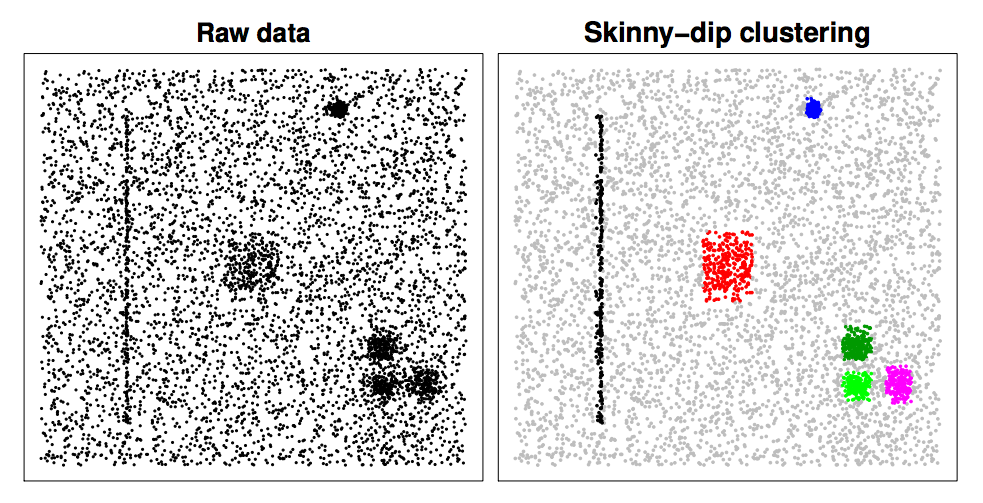
\includegraphics[width=\textwidth]{images/SkinnyDipExample}
\caption{The running example used by Maurus, et al. throughout \cite{skinnydip}}
\label{fig:sdexample}
\end{figure*}

\begin{figure*}[t]
\centering
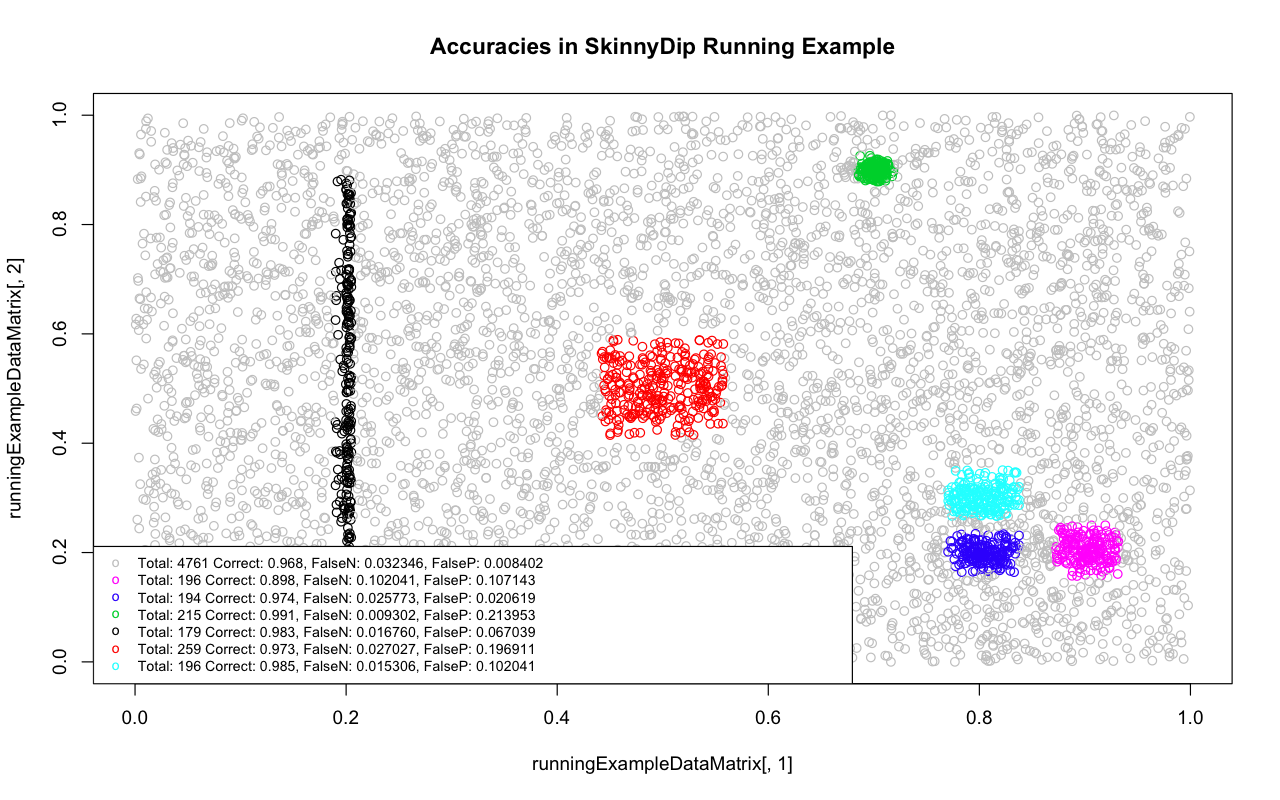
\includegraphics[width=\textwidth]{images/SkinnyDipAccuracy}
\caption{Accuracies of the given SkinnyDip example. NOTE: introduced a bug while updating code that caused legend labels to be shuffled incorrectly, reported data does not correctly match class colors.}
\label{fig:sdaccuracy}
\end{figure*}

\section{Problem Description}
It is not uncommon for some real-world data sets to feature an abundance of noise. Depending on the severity of this noise, classical clustering methods may fail due to due to dependence on clean data or confusion from increasingly excessive noise. SkinnyDip is an algorithm proposed by Maurus et al.\cite{skinnydip} designed to handle clustering data in highly noisy environments. SkinnyDip is based on the statistical concept of the \textit{dip} \cite{dip}. 

The dip views the structure of the Empirical Cumulative Distribution Function(ECDF) of a set of single dimensional data to determine whether it is unimodal or multimodal. This test is expanded to a multidimensional, recursive heuristic in order to isolate the various modes of each feature of a set of data. This results in a deterministic, parameter-free, unsupervised method of finding clusters that are based on the modes of multivariate distributions. 

My goal is to augment the SkinnyDip algorithm with the addition of a Gaussian clustering model in an attempt to reduce the excessive inclusion of noise in hypercubic-bound clusters, and perform additional tests to demonstrate its usefulness on noisy, real-world data sets.


\section{Introduction}
Data clustering is a fundamental problem in Machine Learning, and has been approached in a variety of ways, resulting in a plethora of tools and methods \cite{ClusteringMethods}, many of which are sensitive to noise and other outliers. Additionally, many common techniques, such as k-means clustering, operate as closed set clustering methods and are unable to reject noise at all.

\cite{DBSCAN} is a density-based technique for finding clusters in environments that may contain noise. However, it has the disadvantages of being a parameterized method, and still continues to find extraneous clusters in increasingly noisy data when compared to SkinnyDip.

A single other existing method for clustering using the statistical dip test was found, a technique called DipMeans\cite{dipmeans}. This method takes a different approach to using the dip test by performing it on a collection of distance measurements as opposed to the raw data values themselves. SkinnyDip, however, requires no distance measurements  and is both functionally and computationally distinct from the DipMeans technique.

While SkinnyDip does manage to find all values within a cluster with high accuracy and precision, there is still a notable risk of falsely matching noise to a particular class. This is inherent in the way that the algorithm segments the clusters into hypercubic regions. If the data does not fit a cubic model, then the values included in extreme regions of the cluster (e.g. the corners of a square cluster) are likely to be false positives and should not have been included. This discrepancy increases exponentially as the dimension of the data increases, an issue acknowledged in the original paper\cite{skinnydip}. I plan to demonstrate that the addition of a second step to clustering can reduce this particular error rate, with minimal negative impact on the existing true positive matches.

\section{Data}
A visual example of the purpose of SkinnyDip is demonstrated in the running example data from \cite{skinnydip} (See Figure \ref{fig:sdexample}) which shows the extraction of distinct shapes from a two-dimensional data field that consists of 80\% static noise. A variety of similar clustering methods were shown to perform poorly on this data set, both through the inclusion of the evenly-distributed, static noise in clusters, and through excessive segmentation of the actual classes.

Aside from the uniform background noise, the running example data consists of 2 distinct cluster models: two rectangular model clusters and four 2D Gaussian model clusters. In Figure \ref{fig:sdexample} the square classes are on the left side of the image and are colored red and black, while the remaining four, smaller clusters are the 2D Gaussians. In the process of generating this data, 200 points are generated using their respective distributions (uniform or normal), and placed alongside uniform noise covering the entire field. Any noise that falls within the bounds of these distributions is recategorized as being part of that class.

\section{Progress}
An updated project timeline can be seen in Figure \ref{fig:newmilestones}
\subsection{Completed}
To confirm my suspicion of the high rate of false positive detection in the non-rectangular clusters, I developed some numerical and visual testing tools to 

In my analysis of this synthetic data, it is clear that Gaussian models composed of a large number of false positives, even in just this 2D case. An image analyzing the the classification accuracy of this particular data set is seen in Figure \ref{fig:sdaccuracy}. In this image, the locations of the different clusters are the same, but the coloration has changed slightly, the two leftmost shapes (black and red) are still the rectangularly modeled clusters, and the four, smaller shapes are the 2D Gaussian clusters.

The classes with rectangular models were the only classes that had a false positive rate below 10\%, while the Gaussian modeled classes had false positive ranges that ranged from 10.2\% up to 21.4\%. This supports my hypothesis that the Gaussian modeled clusters would significantly over-sample from their respective classes.


\begin{figure*}[t]
\centering
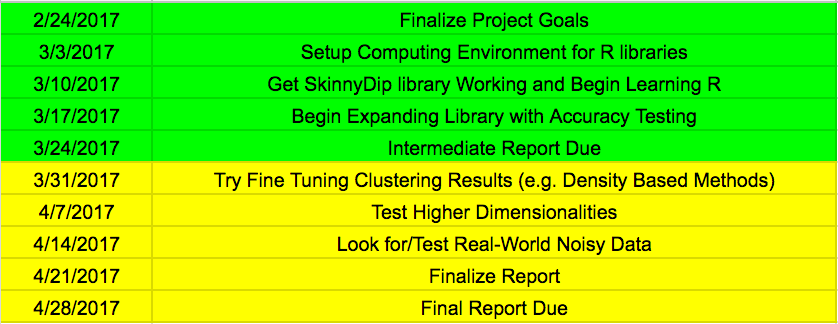
\includegraphics[width=\textwidth]{images/newtimeline}
\caption{Progress on Project Milestones}
\label{fig:newmilestones}
\end{figure*}



\bibliography{intermediate-report}
\bibliographystyle{unsrt}
\end{document}
